\documentclass{midl}

\usepackage{tikz}
\usetikzlibrary{arrows.meta, shapes.geometric, positioning, fit, backgrounds}
\usepackage{enumitem}
\usepackage{float}
\usepackage{xcolor}
\usepackage{amsmath, amssymb}
\usepackage{booktabs}
\usepackage{microtype}
\graphicspath{{../figures/}}

\jmlrvolume{-- Under Review}
\jmlryear{2026}
\jmlrworkshop{Full Paper -- MIDL 2026 submission}

\title[DLMI: Kaggle Challenge]{Deep Learning for Medical Imaging: Out-of-Distribution Histopathology Image Classification}

\midlauthor{
\Name{DEGENEVE Hugo} \Email{hugo.degeneve@student-cs.fr} \and
\Name{KAPOTOS Fotios} \Email{fotiskapotos@gmail.com} \\
\addr{CentraleSupélec}
}

% ============================================================
\begin{document}
\maketitle

\begin{abstract}
We present a solution to the out-of-distribution histopathology image classification
challenge, where models trained on patches from three clinical centers must generalize to
a fully held-out fifth center. Starting from a lightweight DINOv2 embedding baseline with
per-center normalization, we identify the failure modes of frozen-feature approaches and
progressively refine our solution toward end-to-end fine-tuning of KimiaNet equipped with Macenko stain augmentation and Low-Rank Adaptation (LoRA). Macenko augmentation directly addresses the stain-concentration
domain gap by simulating realistic inter-center variability at training time, while LoRA
constrains fine-tuning to a low-rank subspace to prevent overfitting to source-center
styles. The final model achieves $0.95$ accuracy on the held-out validation center and
$0.95$ on the Kaggle test set, compared to $0.90$ for ImageNet-pretrained baselines.
\end{abstract}

\begin{keywords}
domain generalization, histopathology, stain augmentation, LoRA, KimiaNet
\end{keywords}

% ============================================================
\section{Introduction}

Computational pathology relies on models trained at one clinical site being deployed at
another, yet histopathology slides stained and scanned across hospitals exhibit strong
visual variability. This \emph{domain shift} stems from differences in staining protocols,
reagent lots, and scanner hardware, and severely degrades classifier performance on unseen
centers.

Models are trained on patches from three centers (C1, C2, C3), validated on C4, and
evaluated on a held-out fifth center (C5) — a strict \emph{leave-one-domain-out}
generalization problem. Our solution targets the key failure modes of naive fine-tuning
with three components: (i)~\textbf{KimiaNet} \citep{kimianet2021}, a histopathology-pretrained
backbone; (ii)~\textbf{Macenko stain augmentation} \citep{macenko2009}, to simulate
inter-center staining variability at training time; and (iii)~\textbf{LoRA}
\citep{hu2022lora}, to regularize fine-tuning and limit overfitting to source-center styles.

% ============================================================
\section{Exploratory data analysis}

To characterize the domain shift, we applied UMAP (cosine metric, 15 neighbours) to a
10\,000-sample subset of frozen DINOv2 ViT-S/14 embeddings from the three training centers.
Figure~\ref{fig:umap} shows that the centers occupy largely disjoint regions of the 2-D
embedding, while the tumour/normal label boundary does not align with center membership.
This confirms that center identity is a dominant source of variance in the feature space,
directly motivating stain augmentation and a histopathology-specific backbone.

\begin{figure}[H]
\centering
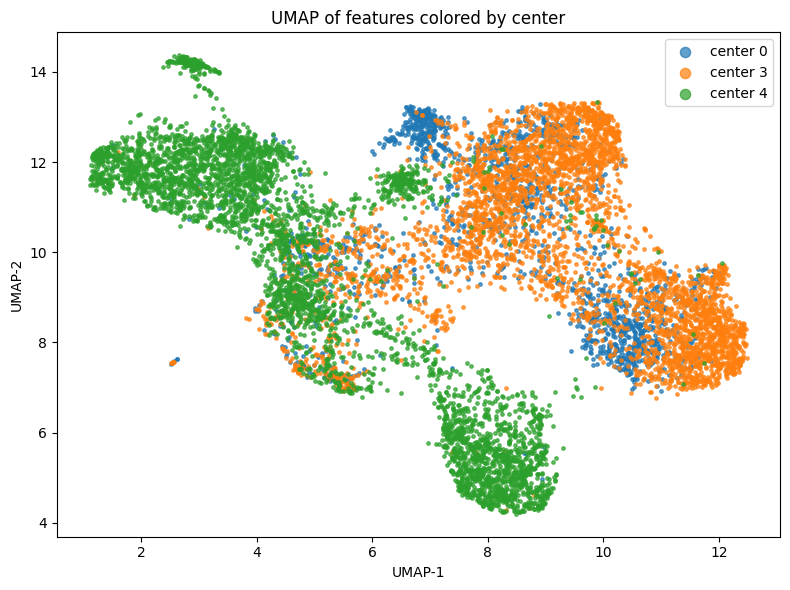
\includegraphics[width=0.48\linewidth]{umap_center.png}\hfill
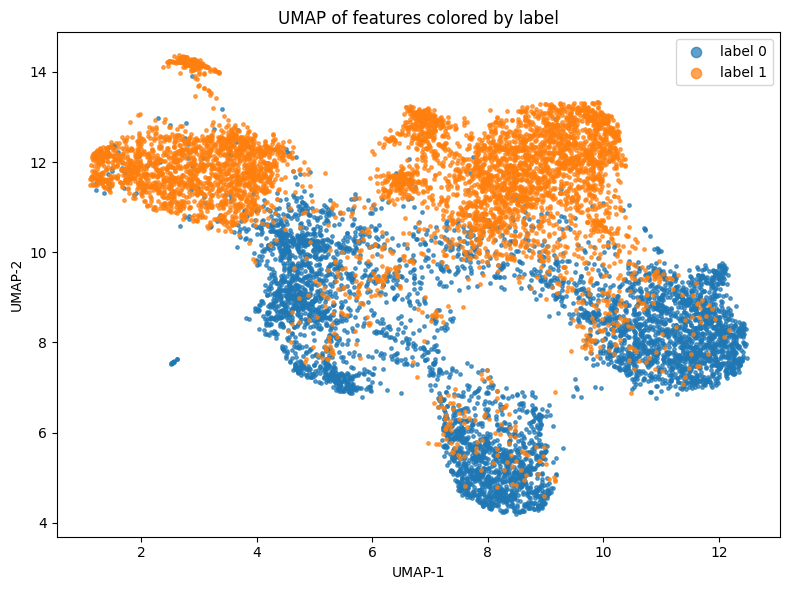
\includegraphics[width=0.48\linewidth]{umap_label.png}
\caption{UMAP of DINOv2 embeddings coloured by center (left) and by label (right).
         Centers cluster separately; the label boundary does not follow center membership.}
\label{fig:umap}
\end{figure}

\section{Architecture and Methodological Components}

\subsection{Backbone: KimiaNet}

\paragraph{Motivation.}
KimiaNet \citep{kimianet2021} is a DenseNet-121 backbone pre-trained on over 240\,000 TCGA
diagnostic slides, giving representations attuned to tissue microstructure and nuclear
morphology rather than scanner-specific artefacts.

\paragraph{Architecture.}
The backbone's final global average pooling layer produces a $1024$-dimensional feature
vector, which is fed into a linear classification head projecting to $K$ classes:
\[
    f_\theta(\mathbf{x}) = W_{\text{cls}}\;\text{GAP}\!\left(\phi_{\text{KimiaNet}}(\mathbf{x})\right) + b_{\text{cls}}.
\]
The full pipeline is illustrated in Figure~\ref{fig:pipeline}.

\begin{figure}[H]
\centering
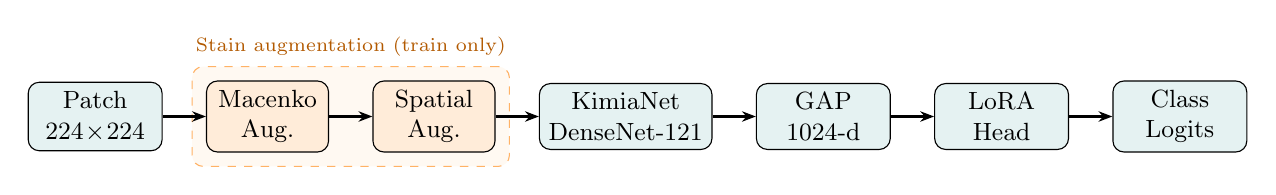
\begin{tikzpicture}[
    node distance=0.4cm and 0.55cm,
    box/.style={draw, rounded corners, minimum height=0.75cm, minimum width=1.7cm,
                font=\small, align=center, fill=teal!10},
    aug/.style={draw, rounded corners, minimum height=0.75cm, minimum width=1.55cm,
                font=\small, align=center, fill=orange!15},
    arrow/.style={-{Stealth[length=5pt]}, thick},
]
\node[box] (input)    {Patch\\$224\!\times\!224$};
\node[aug,  right=of input]      (mac)      {Macenko\\Aug.};
\node[aug,  right=of mac]      (spatial)  {Spatial\\Aug.};
\node[box,  right=of spatial]  (backbone) {KimiaNet\\DenseNet-121};
\node[box,  right=of backbone] (gap)      {GAP\\$1024$-d};
\node[box,  right=of gap]      (lora)     {LoRA\\Head};
\node[box,  right=of lora]     (out)      {Class\\Logits};

\draw[arrow] (input)    -- (mac);
\draw[arrow] (mac)      -- (spatial);
\draw[arrow] (spatial)  -- (backbone);
\draw[arrow] (backbone) -- (gap);
\draw[arrow] (gap)      -- (lora);
\draw[arrow] (lora)     -- (out);

\begin{scope}[on background layer]
  \node[draw=orange!60, dashed, rounded corners, fill=orange!5,
        fit=(mac)(spatial), inner sep=5pt,
        label={[font=\scriptsize, orange!70!black]above:Stain augmentation (train only)}] {};
\end{scope}
\end{tikzpicture}
\caption{Overview of the final pipeline. Orange blocks are applied only at training time.}
\label{fig:pipeline}
\end{figure}

\subsection{Stain Augmentation: Macenko Method}

\paragraph{Motivation.}
Color jitter and standard photometric augmentations operate in RGB space and do not respect
the physics of bright-field staining. Inter-center variability is primarily a
\emph{stain-concentration} effect: the same tissue stained with H\&E at two hospitals
looks similar structurally but differs systematically in hue and saturation. An augmentation
that directly perturbs stain concentrations will therefore generate samples that faithfully
simulate the domain gap, forcing the model to learn stain-invariant features.

\paragraph{Implementation.}
Following \citet{howard2021}, transformations are applied in order: 
(1)~\textbf{Macenko augmentation}: multiplicative perturbation of the stain matrix,
probability $p_{\text{MA}}$; (2)~\textbf{spatial augmentations}: random flips and
$90^{\circ}$ rotations (all orientations are biologically valid); (3)~\textbf{color
jitter}; (4)~\textbf{Gaussian blur} ($p=0.2$, kernel 3); (5)~\textbf{ImageNet
normalization}. 

The Macenko augmentor \citep{macenko2009} fits a $2\times3$ stain matrix $\mathbf{S}$ on each image
via SVD of its optical density point cloud. The two principal stain vectors are
independently perturbed by multiplicative Gaussian noise:
\[
    \tilde{\mathbf{S}}_i = \mathbf{S}_i \cdot \exp(\sigma_i\,\epsilon_i),\quad
    \epsilon_i \sim \mathcal{N}(0,1),\quad i\in\{1,2\},
\]
and the image is reconstructed as $\hat{\mathbf{x}} = I_o\exp(-\mathbf{C}\tilde{\mathbf{S}})$
where $\mathbf{C} = \mathbf{OD}\,\mathbf{S}^{\dagger}$ are the stain concentrations.

\paragraph{Discarded alternatives.}
Macenko stain \emph{normalization} (mapping all patches to a consensus appearance) was
tried but degraded out-of-distribution generalization compared to augmentation. HED
Jitter (additive noise in HED stain-concentration space) was also tested as an alternative to Macenko but was not better than Macenko.

\subsection{Fine-Tuning: Two-Stage LoRA}

\paragraph{Motivation.}
Naive full fine-tuning of KimiaNet on three source centers risks catastrophic forgetting of
generalizable histology features and overfitting to center-specific appearance. LoRA
\citep{hu2022lora} constrains weight updates to a low-rank subspace:
\[
    W = W_0 + \Delta W = W_0 + BA,\quad B\in\mathbb{R}^{d\times r},\;
    A\in\mathbb{R}^{r\times k},\;r\ll\min(d,k),
\]
acting as a structural regularizer that preserves pre-trained features while allowing
task-specific adaptation.

\paragraph{Two-stage recipe.}
\textbf{Stage 1} freezes the entire backbone and trains only the classification head for a
few epochs. This stabilizes the output distribution before any backbone modification.
\textbf{Stage 2} injects LoRA adapters into the linear layers of the DenseNet and unfreezes
the head, training both jointly. The frozen weights $W_0$ are never updated; only $A$, $B$,
and the head are optimized.

% ============================================================
\section{Model Tuning and Comparison}

\subsection{Validation Procedure}

During the initial embedding exploration (Section~\ref{sec:journey}), we used
\textbf{Leave-One-Center-Out CV (LOOCV)} over the three training centers, which is cheap
when only a linear probe is retrained. Once we moved to end-to-end fine-tuning, LOOCV
became impractical, so we switched to \textbf{C4 as a fixed held-out validation center}.
C4 was never used for gradient updates; the final model is selected solely on C4 accuracy.

\subsection{Development Journey}
\label{sec:journey}

\paragraph{Act 1: DINOv2 embedding baseline.}
We began with frozen DINOv2~\citep{oquab2024dinov2} (ViT-S/14) embeddings and a linear
probe evaluated via LOOCV, using per-center feature normalization to mitigate domain shift.
This has a fundamental flaw: center identity is unknown at test time, and frozen
natural-image features encode scanner-specific textures that normalization cannot remove.
The approach failed to generalize and was discarded.

\paragraph{Act 2: End-to-end fine-tuning with stain augmentation.}
We switched to KimiaNet with Macenko stain augmentation, directly simulating inter-center
variability during training. This yielded a substantial C4 improvement
(Table~\ref{tab:ablation}); validation moved to the single held-out C4 center.

\paragraph{Act 3: LoRA regularization.}
Full fine-tuning showed a train–validation gap indicative of overfitting to source-center
styles. LoRA adapters closed this gap and reduced trainable parameters to less than one million. TTA via stain perturbation was tried but did not improve C4 accuracy.

\subsection{Ablation Study}

Table~\ref{tab:ablation} isolates the contribution of each component on C4. All variants
share the same KimiaNet backbone and training budget.

\begin{table}[H]
    \centering
    \small
    \caption{Ablation on validation center C4. Each row adds one component over the previous.}
    \label{tab:ablation}
    \begin{tabular}{lcc}
        \toprule
        \textbf{Configuration} & \textbf{Train Acc.} & \textbf{C4 Acc.} \\
        \midrule
        Head-only + stain augmentation      & 0.85 & 0.75 \\
        Full fine-tune, no augmentation     & 0.98 & 0.89 \\
        Full fine-tune + stain augmentation & 0.97 & 0.93 \\
        LoRA fine-tune + stain augmentation & 0.96 & 0.95 \\
        \bottomrule
    \end{tabular}
\end{table}

\subsection{Preprocessing and Training Details}

\paragraph{Input normalization.}
Images are normalized with ImageNet mean and standard deviation before being fed to the
backbone, consistent with KimiaNet's pre-training protocol.

\paragraph{Class balancing.}
The training set is approximately balanced between the two classes; no re-weighting was
applied.

\subsection{Hyperparameters}

\begin{table}[H]
    \centering
    \small
    \caption{Hyperparameters for each training stage.}
    \label{tab:hyperparams}
    \begin{tabular}{lcc}
        \toprule
        \textbf{Hyperparameter} & \textbf{Stage 1 (head)} & \textbf{Stage 2 (LoRA)} \\
        \midrule
        Optimizer        & AdamW               & AdamW \\
        Learning rate    & $1\times10^{-3}$    & $1\times10^{-3}$ \\
        Weight decay     & $1\times10^{-4}$    & $1\times10^{-4}$ \\
        Batch size       & 512                 & 512 \\
        Epochs           & 1                   & 10 \\
        LR schedule      & Cosine              & Cosine \\
        LoRA rank $r$    & ---                 & 8 \\
        LoRA $\alpha$    & ---                 & 16 \\
        \bottomrule
    \end{tabular}
\end{table}

\subsection{Results and Comparison}

\begin{table}[H]
    \centering
    \small
    \caption{Final performance of our model versus baselines.}
    \label{tab:results}
    \begin{tabular}{lccc}
        \toprule
        \textbf{Model} & \textbf{Train Acc.} & \textbf{C4 Acc.} & \textbf{Kaggle} \\
        \midrule
        ResNet-50 (ImageNet), full FT      & $>0.98$ & 0.92 & 0.90 \\
        ViT-S/16 (DINO), full FT           & $>0.98$ & 0.91 & 0.90 \\
        KimiaNet, head-only + aug.         & 0.85    & 0.75 & ---  \\
        KimiaNet + LoRA + stain aug.       & 0.97    & 0.95 & 0.95 \\
        \bottomrule
    \end{tabular}
\end{table}

\paragraph{Discussion.}
Stain augmentation was the single most impactful component: omitting it limited C4 accuracy
to $0.89$ despite $0.98$ training accuracy, illustrating the severity of stain-based
distribution shift. LoRA added $+0.02$ C4 accuracy while reducing trainable parameters to
$\sim$20\% of full fine-tuning. ResNet-50 and ViT-S/16 baselines were competitive
($0.91$--$0.92$) but outperformed by KimiaNet, confirming the benefit of a
histopathology-specific initialization.

\clearpage
\bibliography{midl-samplebibliography}

\end{document}
